\hsection{Boolean Values}%
\label{sec:bool}%
%
Before, we already mentioned comparisons and their results, which can either be \pythonilIdx{True} or \pythonilIdx{False}.
These two values constitute another basic datatype in \python: \pythonilIdx{bool}.
They are fundamental for making decisions in a program, i.e., for deciding what to do based on data.
%
\hsection{Comparisons}%
%
\begin{figure}%
\centering%
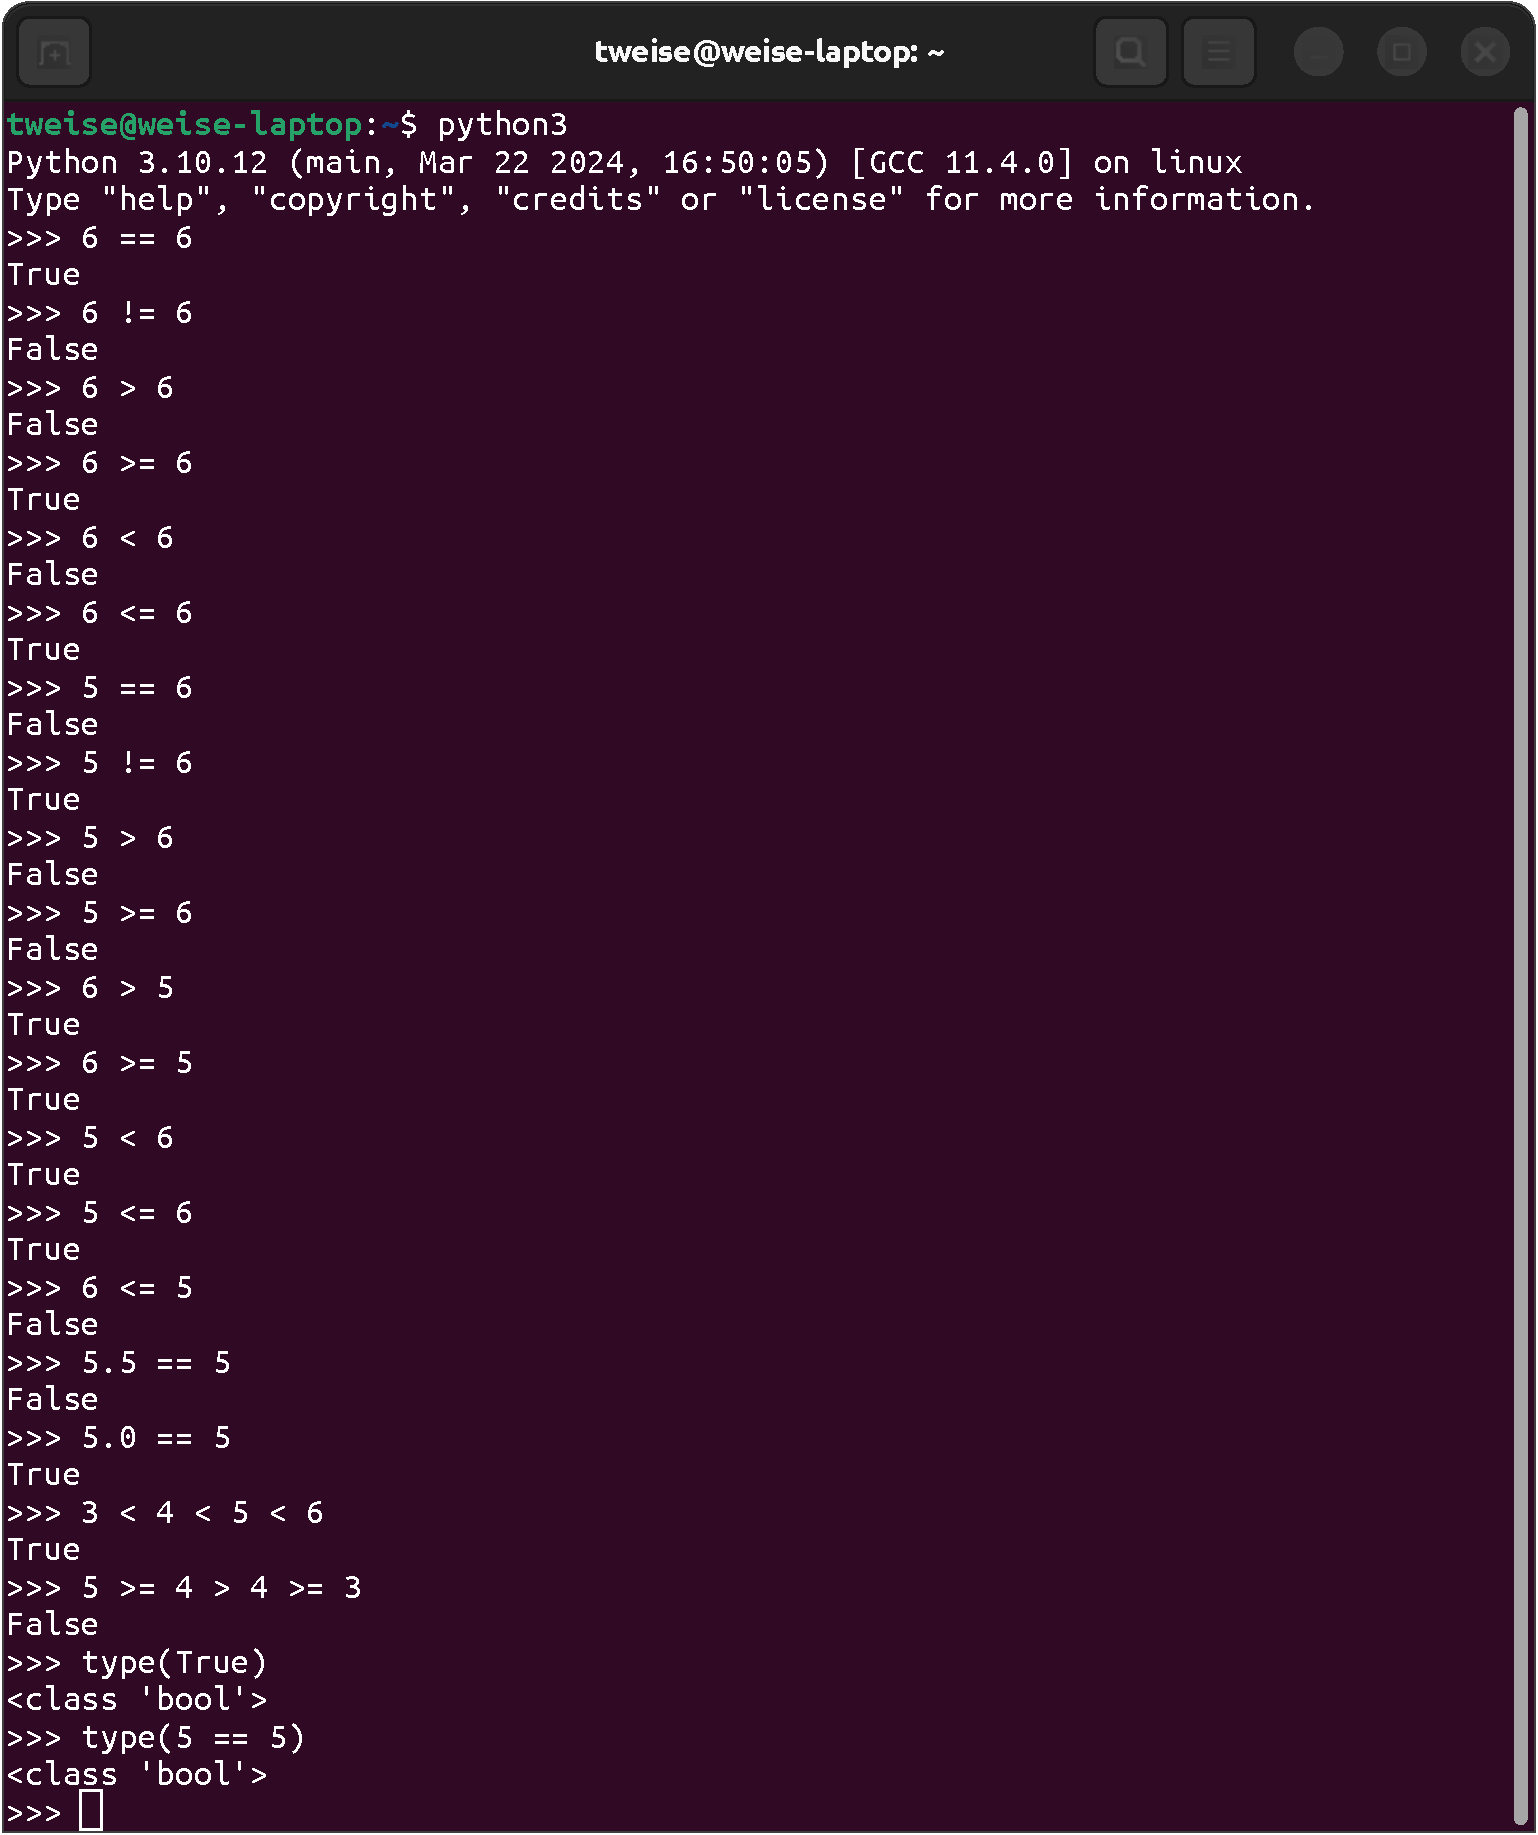
\includegraphics[width=0.8\linewidth]{\currentDir/boolComparisons}%
\caption{The results of basic comparisons are instances of \pythonilIdx{bool}.}%
\label{fig:boolComparisons}%
\end{figure}%
%
In the sections on \pythonilIdx{float}s and \pythonilIdx{int}s, we learned how to do arithmetics with real and integer numbers.
You have learned these operations already in preschool.
However, before you learn to calculate with numbers, you learned how to \emph{compare} them.
If we compare two numbers, the result is either \pythonilIdx{True}, if the comparison works our positively, or \pythonilIdx{False}, if it does not.
\python\ supports six types of comparison:%
%
\begin{itemize}%
%
\item equal: $a = b$ corresponds to \pythonil{a == b}\pythonIdx{==},%
\item unequal: $a \neq b$ corresponds to \pythonil{a != b}\pythonIdx{!=},%
\item less-than: $a < b$ corresponds to \pythonil{a < b}\pythonIdx{<},%
\item less-than or equal: $a \leq b$ corresponds to \pythonil{a <= b}\pythonIdx{<=},%
\item greater-than: $a > b$ corresponds to \pythonil{a > b}\pythonIdx{>}, and%
\item greater-than or equal: $a \geq b$ corresponds to \pythonil{a >= b}\pythonIdx{>=}.%
%
\end{itemize}%
%
How to use these operators is illustrated in \cref{fig:boolComparisons}.
It shows that \pythonil{6 == 6}\pythonIdx{==} yields \pythonilIdx{True}, while \pythonil{6 != 6}\pythonIdx{!=} yields \pythonilIdx{False}.
The expression \pythonil{6 > 6}\pythonIdx{>} gives us \pythonilIdx{False}, but \pythonil{6 >= 6}\pythonIdx{>=} is \pythonilIdx{True}.
\pythonil{6 < 6}\pythonIdx{<} is also \pythonilIdx{False} while \pythonil{6 <= 6} is, of course, \pythonilIdx{True}.
While \pythonil{5 > 6}\pythonIdx{>} is not \pythonilIdx{True}, \pythonil{6 > 5}\pythonIdx{>} is.
It is also possible to compare floating point numbers with integers and vice versa.
\pythonil{5.5 == 5}\pythonIdx{==} is \pythonilIdx{False}, while \pythonil{5.0 == 5} is \pythonilIdx{True}.

Comparisons can also be chained:
\pythonil{3 < 4 < 5 < 6} is \pythonilIdx{True}, because \pythonil{3 < 4} and \pythonil{4 < 5} and \pythonil{5 < 6}.
\pythonil{5 >= 4 > 4 >= 3}, however, is \pythonilIdx{False}, because while \pythonil{5 >= 4} and \pythonil{4 >= 3}, it is not true that \pythonil{4 > 4}.

If we check the type\pythonIdx{type} of \pythonilIdx{True}, it yields \pythonil{<class 'bool'>}, i.e., \pythonilIdx{bool}.
The result of the expression \pythonil{5 == 5} is a \pythonilIdx{bool} as well.

When talking about comparisons, there is one important, counter-intuitive exception to recall:
The \pythonilIdx{nan}\pythonIdx{Not a Number} floating point value\pythonIdx{float} from \cref{sec:float:special}.
In \cref{fig:floatMathInConsoleNaN}, we learned that \pythonil{nan == nan}\pythonIdx{==} is \pythonilIdx{False} and \pythonil{nan != nan}\pythonIdx{!=} is \pythonilIdx{True}.
This is the only primitive value (to my knowledge) which is not equal to itself.%
\endhsection%
%
%
\hsection{Boolean Operators}%
%
\begin{figure}%
\centering%
%
\subfloat[][%
The truth table for the logical conjunction\pythonIdx{bool!conjunction} (\emph{logical and}\pythonIdx{and}): \pythonil{a and b}.%
\label{fig:booleanAnd}%
]{%
~~~~%
\begin{tabular}{|c|c|c|}%
\hline%
\pythonil{a}&\pythonil{b}&\pythonil{a and b}\\%
\hline%
\pythonilIdx{False}&\pythonilIdx{False}&\pythonilIdx{False}\\%
\hline%
\pythonilIdx{False}&\pythonilIdx{True}&\pythonilIdx{False}\\%
\hline%
\pythonilIdx{True}&\pythonilIdx{False}&\pythonilIdx{False}\\%
\hline%
\pythonilIdx{True}&\pythonilIdx{True}&\pythonilIdx{True}\\%
\hline%
\end{tabular}%
~~~~%
}%
%
\strut\hfill\strut%
%
\subfloat[][%
The truth table for the logical disjunction\pythonIdx{bool!disjunction} (\emph{logical or})\pythonIdx{or}: \pythonil{a or b}.%
\label{fig:booleanOr}%
]{%
~~~~%
\begin{tabular}{|c|c|c|}%
\hline%
\pythonil{a}&\pythonil{b}&\pythonil{a or b}\\
\hline%
\pythonilIdx{False}&\pythonilIdx{False}&\pythonilIdx{False}\\%
\hline%
\pythonilIdx{False}&\pythonilIdx{True}&\pythonilIdx{True}\\%
\hline%
\pythonilIdx{True}&\pythonilIdx{False}&\pythonilIdx{True}\\%
\hline%
\pythonilIdx{True}&\pythonilIdx{True}&\pythonilIdx{True}\\%
\hline%
\end{tabular}%
~~~~%
}%
%
\strut\hfill\strut%
%
\subfloat[][%
The truth table for the logical negation\pythonIdx{bool!negation} (\emph{logical not}\pythonIdx{not}): \pythonil{not a}.%
\label{fig:booleanNot}%
]{%
~~~~%
\begin{tabular}{|c|c|}%
\hline%
\pythonil{a}&\pythonil{not a}\\%
\hline%
\pythonilIdx{False}&\pythonilIdx{True}\\%
\hline%
\pythonilIdx{True}&\pythonilIdx{False}\\%
\hline%
\end{tabular}%
~~~~%
}%
%
\caption{The truth tables for the Boolean operators \pythonilIdx{and}, \pythonilIdx{or}, and \pythonilIdx{not}.}%
\label{fig:boolLogicTables}%
\end{figure}%
%
\begin{figure}%
\centering%
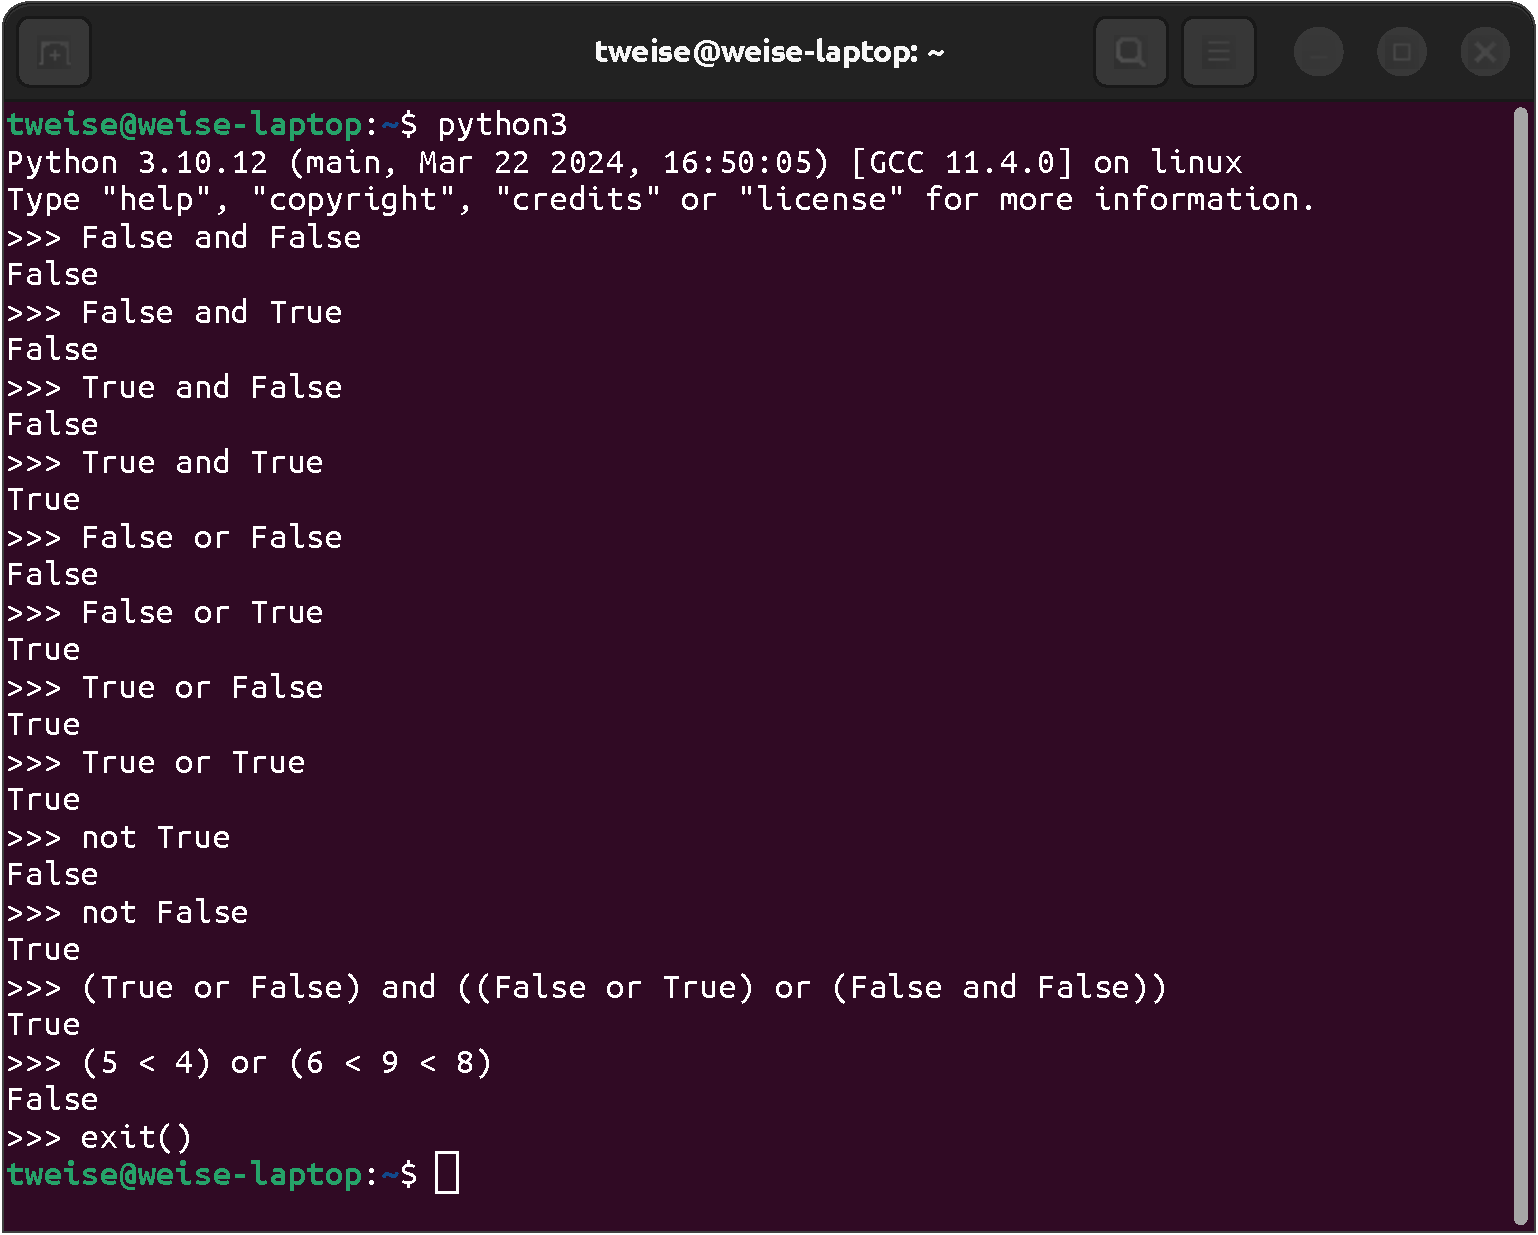
\includegraphics[width=0.8\linewidth]{\currentDir/boolLogic}%
\caption{The \pythonilIdx{bool} values can be combined with the Boolean logical operators \pythonilIdx{and}, \pythonilIdx{or}, and \pythonilIdx{not}.}%
\label{fig:boolLogic}%
\end{figure}%
%
The most common operations with Boolean values are the well-known Boolean logical operators \pythonilIdx{and}, \pythonilIdx{or}, and \pythonilIdx{not}.
Their truth tables are illustrated in \cref{fig:boolLogicTables}.%
%
\begin{itemize}%
%
\item A Boolean conjunction\pythonIdx{bool!conjunction}, i.e., \pythonilIdx{and}, is \pythonilIdx{True} if and only both of its operands are also \pythonilIdx{True} and \pythonilIdx{False} otherwise, as shown in \cref{fig:booleanAnd}.%
%
\item A Boolean disjunction\pythonIdx{bool!disjunction}, i.e., \pythonilIdx{and}, is \pythonilIdx{True} if at least one of its two operands is \pythonilIdx{True} and \pythonilIdx{False} otherwise, as shown in \cref{fig:booleanOr}.%
%
\item The Boolean negation\pythonIdx{bool!negation}, i.e., \pythonilIdx{not}, is \pythonilIdx{True} if its operand is \pythonilIdx{False}. %
Otherwise, it is \pythonilIdx{False}, as shown in \cref{fig:booleanNot}.%
%
\end{itemize}%
%
\begin{sloppypar}%
In \cref{fig:boolLogic} we explore these three operators in the \python\ console.
You can see that the operations can be used exactly as in the truth tables and yield the expected results.
Additionally, you can of course nest and combine Boolean operators using parentheses\pythonIdx{(}\pythonIdx{)}.
For example, \pythonil{(True or False) and ((False or True) or (False and False))} resolves to \pythonil{True and (True or False)}, which becomes \pythonil{True and True}, which ultimately becomes \pythonilIdx{True}.
You can also combine Boolean expressions like comparisons using the logical operators:
\pythonil{(5 < 4) or (6 < 9 < 8)} will be resolved to \pythonil{(False) or (False)}, which becomes \pythonilIdx{False}.%
\end{sloppypar}%
%
\endhsection%
%
\hsection{Summary}%
%
Boolean values are very easy to understand and deal with.
They can either be \pythonilIdx{True} or \pythonilIdx{False}.
They can be combined using \pythonilIdx{and}, \pythonilIdx{or}, and \pythonilIdx{not}.
And, finally, they are the results of comparison operators.
Later, we will learn that Boolean decisions form the foundation for steering the control flow of programs.%
%
\endhsection%
\endhsection%
%
